\documentclass[11pt]{article}
\usepackage[margin=1in]{geometry}
\usepackage{graphicx}
\usepackage{booktabs}
\usepackage{hyperref}
\usepackage{amsmath}
\title{Harness Optimization for Graph Reasoning: Learn Small, Run Big}
\author{Bikash Kumar Paul \and Abdullah Al Noman \and Samin Rahman Khan \and Md Zarzees Uddin Shah Chowdhury}
\date{CS 5624, December 2026}

\begin{document}
\maketitle

% Course policy: the prose below must be written by the authors. This file is a
% skeleton that points to the generated tables and figures only.

\begin{abstract}
% TODO: human-written abstract.
\end{abstract}

\section{Introduction}
% TODO: research question, contributions, motivation.

\section{Related Work}
% TODO: harness optimization, graph reasoning benchmarks, GraphArena, GraphQA.

\section{Problem Setup}
% TODO: tasks, splits, harness definition, answer protocol, metrics.
Tasks implemented: shortest path, connected components, cycle detection,
diameter, reachability, max clique, Hamiltonian path, common neighbors, MIS,
MVC, GED, MCS, TSP, and the GraphQA scalar/classification/flow tasks.
See \texttt{experiments/BENCHMARK\_COVERAGE.md} for the coverage matrix.

% >>> AI-DRAFT (E15, 2026-11-21): rewrite before submission
\paragraph{Setup facts.}
Actor: Qwen3-4B-Instruct-2507 (snapshot \texttt{cdbee75f}, BF16, vLLM 0.34.0),
temperature 0, 8{,}192-token context unless stated otherwise. Synthetic
splits: train 300, val 150, \texttt{test\_small} 150, \texttt{test\_medium}
150, \texttt{test\_large} 100, \texttt{test\_stress} 50; node ranges 4--50,
100--299, 501--997 and 2{,}000. The fresh held-out split
\texttt{test\_small\_fresh} has 150 problems (seed 56240) and zero graph
overlap with the six frozen splits. Real benchmarks: GraphArena easy and hard
at 100 problems per task and GraphQA test at 50 per task, taken in adapter
order; the original 20/task records are a subset. Harnesses: Baseline A
(minimal protocol), Baseline B (expert rules) and Baseline B v2 (14 rules).
Tool runs use a Python/NetworkX sandbox with a 30\,s timeout, a 2\,GB memory
cap and an 8-step limit. The model must put its final answer in
\texttt{<answer>...</answer>}; scoring checks feasibility and then the
task-specific exact answer. Reported metrics are accuracy, parsed rate,
feasible rate, tokens and wall time. Every synthetic cell for A/B/v2 has three
repeats; values are mean $\pm$ population std.
% <<< AI-DRAFT

\section{Baselines and Harnesses}
% TODO: Baseline A, Baseline B, Baseline B v2, H* selection.
\begin{table}[h]
\centering
\begin{tabular}{lrr}
\toprule
Harness & test\_small (150, k=3) & notes \\
\midrule
Baseline A & 89.3 $\pm$ 1.6\% & minimal protocol \\
Baseline B & 94.4 $\pm$ 0.6\% & original expert rules \\
Baseline B v2 (13 rules) & 93.3\% & pilot-tuned, single run \\
Baseline B v2 (14 rules) & 95.8 $\pm$ 1.4\% & full scaling harness \\
\bottomrule
\end{tabular}
\caption{Synthetic \texttt{test\_small} results, Qwen3-4B BF16 on one B200.
Values with $\pm$ are mean and population std over three repeats; the 13-rule
v2 value is the original single run and was not repeated.}
\end{table}

\section{Small-Graph Optimization}
% TODO: SkillOpt/GEPA loop, accepted/rejected edits, why no candidate improved.
Two optimizer runs (8 rounds from v2, 10 rounds from A) rejected every
candidate. The validation gate prevented regressions; v2 is frozen as
$H^*_{\text{small}}$.

\section{Scaling Results}
% TODO: full scaling curves and delta_gen.
\begin{figure}[h]
\centering
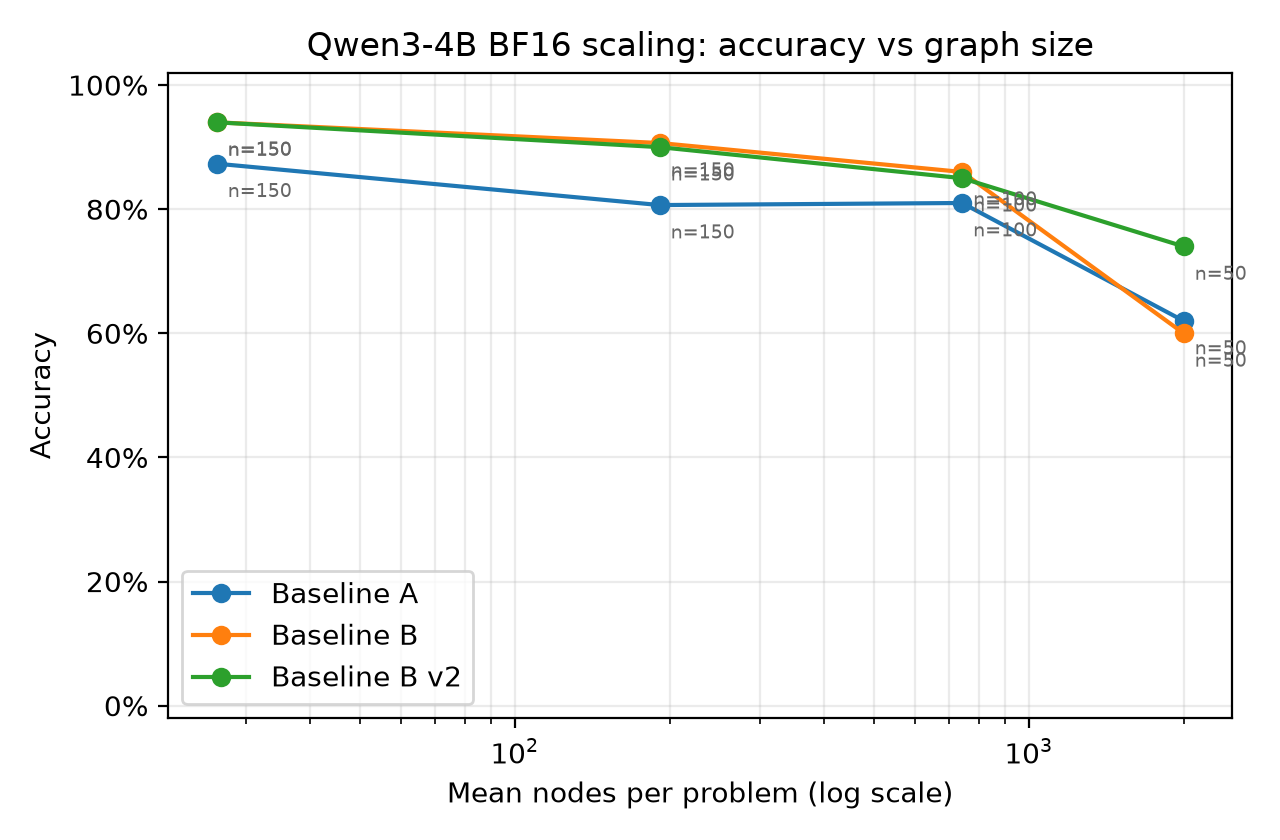
\includegraphics[width=0.85\linewidth]{figures/scaling_4b_accuracy_vs_size.png}
\caption{Accuracy versus graph size for Baselines A/B/B v2.}
\end{figure}

\begin{table}[h]
\centering
\begin{tabular}{lrrrr}
\toprule
Harness & small & medium & large & stress \\
\midrule
Baseline A & 89.3 $\pm$ 1.6 & 86.2 $\pm$ 3.9 & 84.3 $\pm$ 2.4 & 66.0 $\pm$ 2.8 \\
Baseline B & 94.4 $\pm$ 0.6 & 92.0 $\pm$ 1.1 & 90.7 $\pm$ 3.7 & 72.7 $\pm$ 9.0 \\
Baseline B v2 & 95.8 $\pm$ 1.4 & 90.7 $\pm$ 0.9 & 85.3 $\pm$ 0.5 & 73.3 $\pm$ 0.9 \\
\bottomrule
\end{tabular}
\caption{Full synthetic scaling accuracy (\%): mean and population std over
three repeats. The same data appear with $n$ per split in the final-results
section.}
\end{table}

\section{Rule Ablations}
% TODO: interpret test\_large, test\_stress, and val ablations.
See \texttt{experiments/qwen3\_4b\_ablation\_*/ablation/ablation\_summary.txt}
and \texttt{report/tables/ablation\_*.csv}.

\section{Real Benchmark Evaluation}
% TODO: GraphArena/GraphQA results and error analysis.
GraphArena (20 problems/task): easy 74.5\%, hard 61.0\%.
GraphQA test (20/task): 88.3\%.
See \texttt{experiments/qwen3\_4b\_real\_bench/}.

\section{Discussion and Limitations}
% TODO: synthetic vs real benchmarks, scale, model choice, sandbox assumptions,
% test\_small tuning caveat, source-answer caveat for maximum flow and node
% classification.

\section{Conclusion}
% TODO: human-written conclusion.

\bibliographystyle{plain}
% \bibliography{references}


% >>> AI-DRAFT (E15, 2026-11-21): rewrite before submission
\section{Final experimental results}
This section is a factual integration of the final experiments. The full
methods and tables are in \texttt{report/EXPERIMENTAL\_REPORT.md}; the authors
should rewrite this prose.

\paragraph{Tool access.}
Python/NetworkX tool access changes the task substantially. Over three
repeats at the original 8k context, Baseline B v2 scores
96.4 $\pm$ 0.3\% with tools and 35.8 $\pm$ 0.6\% without them on
\texttt{test\_small}; on \texttt{test\_medium} the two conditions are
91.1 $\pm$ 1.9\% and 15.3 $\pm$ 0.5\%. On the 25-problem
\texttt{test\_large} subset used by the original tool study, v2 scores
92.0 $\pm$ 3.3\% with tools and 0.0\% without tools in all three repeats;
the no-tools prompts exceed the 8k limit. Baseline A shows the same pattern
(90.4 $\pm$ 0.8\% versus 39.6 $\pm$ 2.8\% on small).
Table~\ref{tab:tool-access}
and Figure~\ref{fig:tool-access} summarize this. The C/gcc backend without a
graph library scores 12.0\% on 25 small problems (one pilot run).

\begin{figure}[h]
\centering
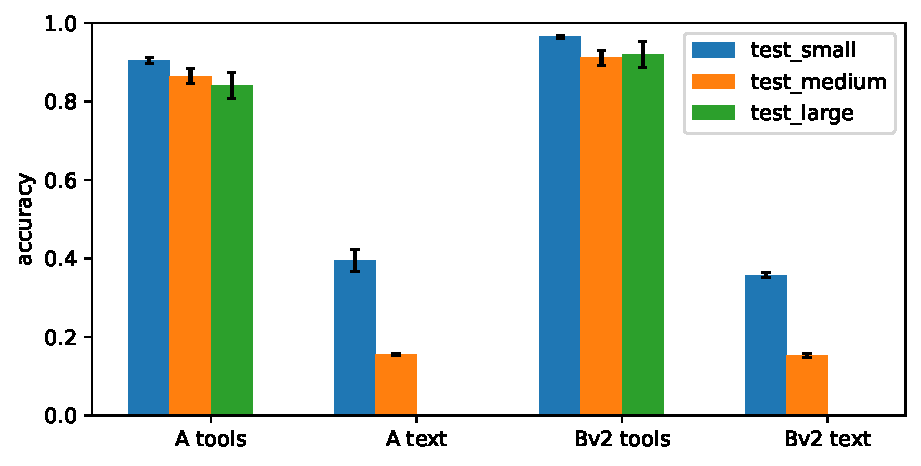
\includegraphics[width=0.85\linewidth]{figures/fig_tool_access.pdf}
\caption{Tool access versus no-tools accuracy.}
\label{fig:tool-access}
\end{figure}

\begin{table}[h]
\centering
\begin{tabular}{lrrr}
\toprule
condition & small (n=150) & medium (n=150) & large (n=25) \\
\midrule
a\_tools & 90.4\% $\pm$ 0.8 & 86.4\% $\pm$ 1.9 & 84.0\% $\pm$ 3.3 \\
a\_text & 39.6\% $\pm$ 2.8 & 15.6\% $\pm$ 0.3 & 0.0\% $\pm$ 0.0 \\
b\_v2\_tools & 96.4\% $\pm$ 0.3 & 91.1\% $\pm$ 1.9 & 92.0\% $\pm$ 3.3 \\
b\_v2\_text & 35.8\% $\pm$ 0.6 & 15.3\% $\pm$ 0.5 & 0.0\% $\pm$ 0.0 \\
\bottomrule
\end{tabular}

\caption{Accuracy by tool condition and graph split.}
\label{tab:tool-access}
\end{table}

\paragraph{Held-out small-graph estimate.}
A fresh small split (\texttt{test\_small\_fresh}, seed 56240, 30 problems per
task, 150 total, zero graph overlap with the six frozen splits) was run three
times per harness. Accuracy is Baseline A 88.4 $\pm$ 1.3\%, Baseline B
93.8 $\pm$ 0.8\%, and Baseline B v2 95.8 $\pm$ 0.8\% (Table~\ref{tab:heldout}).
The contaminated \texttt{test\_small} value for v2 was 94.0\%, so the held-out
estimate is not lower. Per task, v2 improves cycle detection over B
(95.6\% versus 82.2\%) and is lower on max clique (83.3\% versus 88.9\%).
McNemar B versus v2 gives $p=1.00$, $0.34$, $0.30$ in the three repeats.

\begin{table}[h]
\centering
\begin{tabular}{lrrcr}
\toprule
harness & repeats & accuracy & std (pp) & 95\% Wilson CI \\
\midrule
baseline\_a & 3 & 88.4\% & 1.3 & [85.2\%, 91.1\%] \\
baseline\_b & 3 & 93.8\% & 0.8 & [91.2\%, 95.7\%] \\
baseline\_b\_v2 & 3 & 95.8\% & 0.8 & [93.5\%, 97.3\%] \\
\bottomrule
\end{tabular}

\caption{Accuracy on the fresh held-out small split, 3 repeats.}
\label{tab:heldout}
\end{table}

\paragraph{Scaling and ablation.}
Table~\ref{tab:main-scaling} and Figure~\ref{fig:scaling} show the synthetic
scaling results as mean $\pm$ std over three repeats. v2 is higher than B on
small (95.8 $\pm$ 1.4 versus 94.4 $\pm$ 0.6), the two are within 1.5 points on
medium and on the 2,000-node stress split, and B is higher on large
(90.7 $\pm$ 3.7 versus 85.3 $\pm$ 0.5). The large difference is significant in
repeat 2 (McNemar $p=0.006$) and not in repeats 1 and 3 ($p=1.00$, $0.18$).
The small-minus-large gap is 10.4 $\pm$ 0.8 points for v2, 3.8 $\pm$ 2.2 for B,
and 5.0 $\pm$ 1.7 for A. Rule ablations are in
Table~\ref{tab:rule-ablation}.

\begin{figure}[h]
\centering
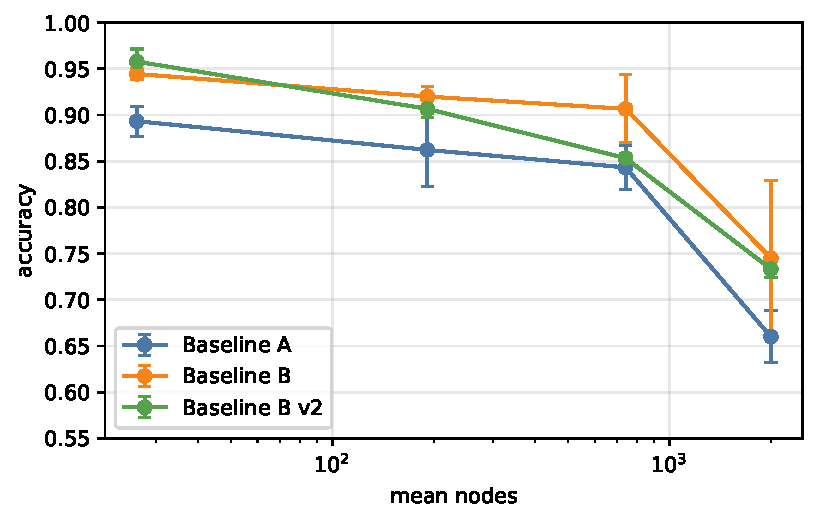
\includegraphics[width=0.85\linewidth]{figures/fig_scaling.pdf}
\caption{Accuracy versus graph size.}
\label{fig:scaling}
\end{figure}

\begin{table}[h]
\centering
\begin{tabular}{lrrrrr}
\toprule
Harness & small & medium & large & stress & n \\
\midrule
baseline\_a & 89.3\% $\pm$ 1.6 & 86.2\% $\pm$ 3.9 & 84.3\% $\pm$ 2.4 & 66.0\% $\pm$ 2.8 & 150 \\
baseline\_b & 94.4\% $\pm$ 0.6 & 92.0\% $\pm$ 1.1 & 90.7\% $\pm$ 3.7 & 72.7\% $\pm$ 9.0 & 150 \\
baseline\_b\_v2 & 95.8\% $\pm$ 1.4 & 90.7\% $\pm$ 0.9 & 85.3\% $\pm$ 0.5 & 73.3\% $\pm$ 0.9 & 150 \\
\bottomrule
\end{tabular}

\caption{Full synthetic scaling accuracy.}
\label{tab:main-scaling}
\end{table}

\begin{table}[h]
\centering
\small
\begin{tabular}{rrrp{7cm}}
\toprule
rule & accuracy & delta & text \\
\midrule
0 & 89.0\% & -4.0\% & Use the NetworkX `G` object directly; never infer edges or distances f \\
1 & 88.0\% & -3.0\% & Prefer exact library routines: nx.shortest\_path, nx.connected\_componen \\
2 & 88.0\% & -3.0\% & For maximum clique, run exact search only when the graph is small; on  \\
3 & 86.0\% & -1.0\% & Check feasibility before answering: path endpoints and edges, one repr \\
4 & 89.0\% & -4.0\% & Keep sandbox output short: print only the result, its length/size, and \\
5 & 86.0\% & -1.0\% & If code times out or errors, change the algorithm instead of rerunning \\
6 & 83.0\% & +2.0\% & Put only the final node list inside <answer></answer>; use [] for a ne \\
7 & 86.0\% & -1.0\% & For connected components, print `list(nx.connected\_components(G))` and \\
8 & 90.0\% & -5.0\% & For diameter, find a pair of nodes whose shortest-path distance equals \\
9 & 90.0\% & -5.0\% & Always call print(...) on the value you need. The sandbox also echoes  \\
10 & 89.0\% & -4.0\% & For maximum clique on small graphs, print `nx.max\_weight\_clique(G, wei \\
11 & 89.0\% & -4.0\% & Once a successful run prints a feasible result, stop and give that res \\
12 & 87.0\% & -2.0\% & Never filter, sort, or index nodes by numeric value; node ids are arbi \\
13 & 88.0\% & -3.0\% & Materialize NetworkX generators with list(...) or dict(...) before ite \\
\bottomrule
\end{tabular}

\caption{Rule ablation on full \texttt{test\_large}.}
\label{tab:rule-ablation}
\end{table}

\paragraph{Real benchmarks.}
Table~\ref{tab:real-bench} reports the GraphArena and GraphQA results for
Baseline B v2. GED, MCS, TSP and hard MIS are the main failures.

\begin{table}[h]
\centering
\begin{tabular}{lrrrr}
\toprule
benchmark & n & accuracy & parsed & feasible \\
\midrule
GraphArena easy & 200 & 74.5\% & 95.0\% & 84.0\% \\
GraphArena hard & 200 & 61.0\% & 97.5\% & 83.5\% \\
GraphQA test & 240 & 88.3\% & 100.0\% & 99.2\% \\
\bottomrule
\end{tabular}

\caption{Real benchmark accuracy at 20 problems per task.}
\label{tab:real-bench}
\end{table}

\paragraph{Characteristics.}
Table~\ref{tab:characteristics} and Figures~\ref{fig:characteristics} and
\ref{fig:density} break accuracy down by graph family, density and size for A,
B and v2 on the 450 frozen scaling problems. A logistic regression
(\texttt{correct} $\sim \log n$ + density + task + harness) gives an odds ratio
of 0.63 per unit $\log n$ (95\% CI 0.55--0.72), 0.76 per 0.1 density
(0.64--0.90), and 1.91 for v2 versus A (1.29--2.81). Family and task are
perfectly nested in this generator (tree only occurs with cycle detection,
mixed only with connected components), so their effects are not separately
identified.

\begin{figure}[h]
\centering
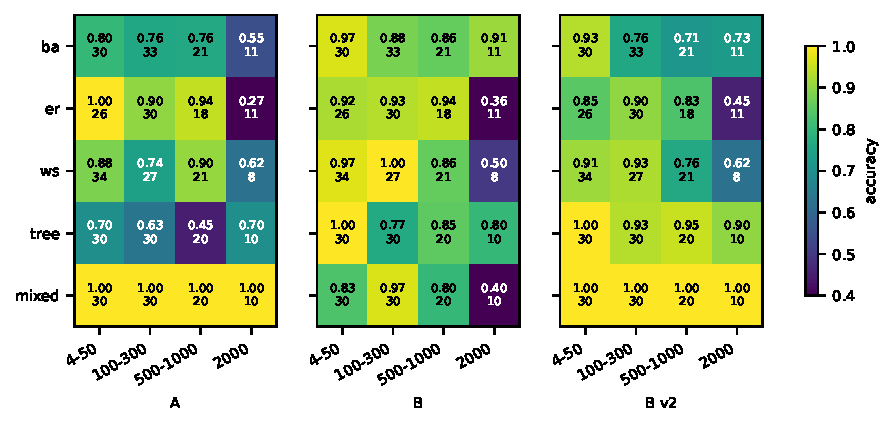
\includegraphics[width=0.9\linewidth]{figures/fig_characteristics.pdf}
\caption{Accuracy by graph family for each harness.}
\label{fig:characteristics}
\end{figure}

\begin{figure}[h]
\centering
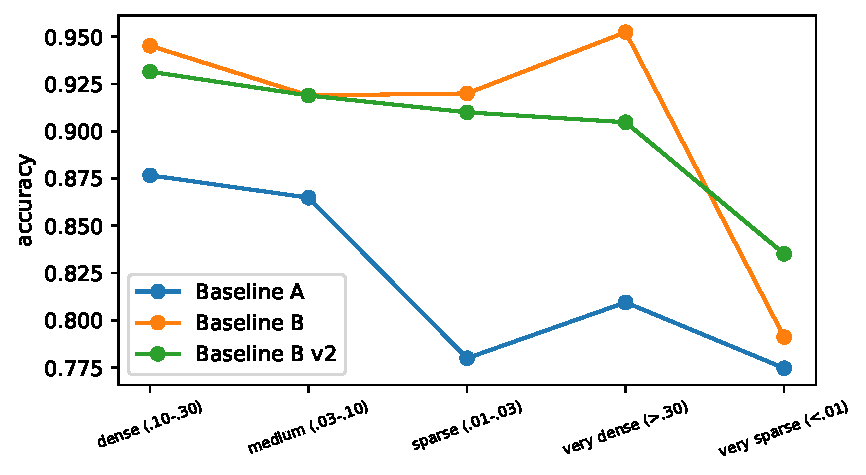
\includegraphics[width=0.85\linewidth]{figures/fig_density.pdf}
\caption{Accuracy by density bin for each harness.}
\label{fig:density}
\end{figure}

\begin{table}[h]
\centering
\begin{tabular}{lrrr}
\toprule
harness & family & n & accuracy \\
\midrule
Baseline A & ba & 95 & 74.7\% \\
Baseline A & er & 85 & 85.9\% \\
Baseline A & mixed & 90 & 100.0\% \\
Baseline A & tree & 90 & 62.2\% \\
Baseline A & ws & 90 & 82.2\% \\
Baseline B & ba & 95 & 90.5\% \\
Baseline B & er & 85 & 85.9\% \\
Baseline B & mixed & 90 & 82.2\% \\
Baseline B & tree & 90 & 86.7\% \\
Baseline B & ws & 90 & 91.1\% \\
Baseline B v2 & ba & 95 & 80.0\% \\
Baseline B v2 & er & 85 & 81.2\% \\
Baseline B v2 & mixed & 90 & 100.0\% \\
Baseline B v2 & tree & 90 & 95.6\% \\
Baseline B v2 & ws & 90 & 85.6\% \\
\bottomrule
\end{tabular}

\caption{Accuracy by graph family, all frozen scaling splits.}
\label{tab:characteristics}
\end{table}

\paragraph{Optimization and proxies.}
All automated optimizers (SkillOpt-style, GEPA, RRSI, Meta-Harness) accepted
zero improving edits in the final pilot. Table~\ref{tab:costs} reports their
token/time cost. Figure~\ref{fig:optimizer-curves} shows the best validation
accuracy versus cumulative tokens. Measured evaluation cost rises from
2.8\,s and 4.7k tokens per problem on small graphs to 3.8\,s and 5.0k tokens
on large graphs. A 10-round optimization run that used large graphs directly
is therefore estimated at 3.52M tokens and 0.74 GPU-hours, 1.94$\times$ the
average completed small-graph run (Table~\ref{tab:cost-counterfactual}); cost
alone does not explain optimizing on small graphs.

\paragraph{Proxies for large-graph accuracy.}
On the same 15 rule-ablation candidates, the learned static proxy (static
harness-text features, leave-one-out) reaches Spearman $-0.25$ (95\% CI
$-0.73$ to $0.41$) against val accuracy and $0.29$ ($-0.36$ to $0.85$) against
\texttt{test\_large}; with $n=15$ neither is distinguishable from zero, and
top-3 recall is zero for both (Table~\ref{tab:proxy},
Figure~\ref{fig:proxy}). On the earlier pool of 18 optimizer candidates the
same proxy reached $0.553$ against val; that pool varies the prompt and rule
list much more than one-rule ablations do. A cheap rollout with one problem
per task reached $-0.17$ against val on the 18-candidate pool.

\begin{figure}[h]
\centering
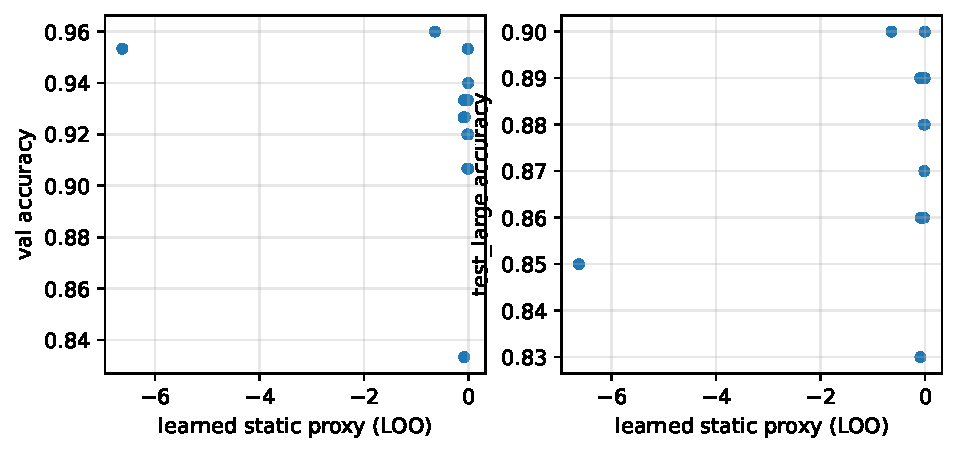
\includegraphics[width=0.9\linewidth]{figures/fig_proxy.pdf}
\caption{Learned static proxy versus val and \texttt{test\_large} accuracy on
the same 15 candidates.}
\label{fig:proxy}
\end{figure}

\begin{table}[h]
\centering
\small
\begin{tabular}{llrlrrlp{2.2cm}}
\toprule
proxy & target & n & Spearman & 95\% CI & pairwise & top-3 & pool \\
\midrule
static-LOO & val & 18 & 0.55 & -- & 70.1\% & -- & earlier-18 \\
rollout-k1 & val & 18 & -0.17 & -- & 58.2\% & 0 & earlier-18, k=1 \\
static-LOO & val & 15 & -0.25 & [-0.73, 0.41] & 37.0\% & 0 & same-15 \\
static-LOO & large & 15 & 0.29 & [-0.36, 0.85] & 71.4\% & 0 & same-15 \\
\bottomrule
\end{tabular}

\caption{Proxy ranking quality by proxy, target and candidate pool.}
\label{tab:proxy}
\end{table}

\begin{figure}[h]
\centering
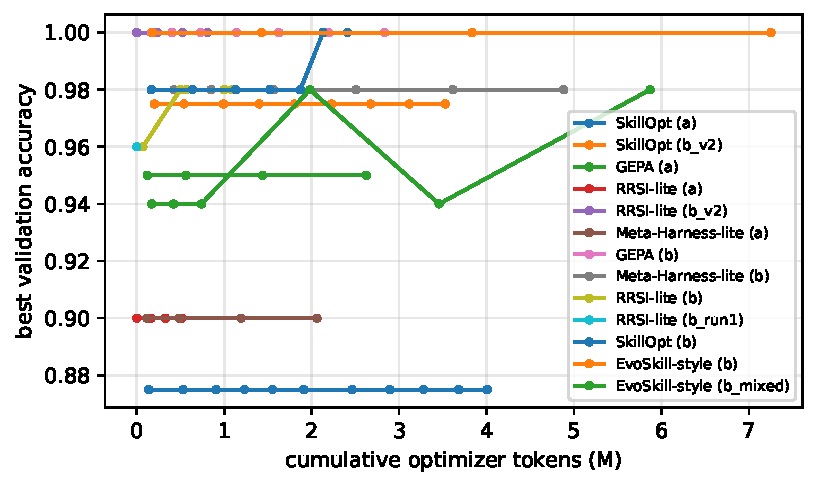
\includegraphics[width=0.8\linewidth]{figures/fig_optimizer_curves.pdf}
\caption{Best validation accuracy versus cumulative optimizer tokens.}
\label{fig:optimizer-curves}
\end{figure}

\begin{table}[h]
\centering
\small
\begin{tabular}{llrrrrr}
\toprule
optimizer & start & tokens (M) & wall s & GPU-h & USD tokens & USD GPU-h \\
\midrule
SkillOpt & baseline\_a & 4.01 & 486 & 0.14 & USD 2.80 & USD 0.54 \\
SkillOpt & baseline\_b\_v2 & 3.53 & 383 & 0.11 & USD 2.47 & USD 0.43 \\
GEPA & baseline\_a & 1.19 & 597 & 0.17 & USD 0.83 & USD 0.66 \\
RRSI-lite & baseline\_a & 0.51 & 426 & 0.12 & USD 0.36 & USD 0.47 \\
RRSI-lite & baseline\_b\_v2 & 0.81 & 405 & 0.11 & USD 0.57 & USD 0.45 \\
Meta-Harness-lite & baseline\_a & 0.87 & 426 & 0.12 & USD 0.61 & USD 0.47 \\
\bottomrule
\end{tabular}

\caption{Optimizer token, time and estimated dollar cost.}
\label{tab:costs}
\end{table}

\begin{table}[h]
\centering
\small
\begin{tabular}{lrrrrr}
\toprule
training graphs & tok/prob & s/prob & 10-round tokens (M) & GPU-h & ratio vs measured run \\
\midrule
small & 4731 & 2.8 & 3.31 & 0.54 & 1.82 \\
medium & 4617 & 3.4 & 3.23 & 0.66 & 1.78 \\
large & 5029 & 3.8 & 3.52 & 0.74 & 1.94 \\
\bottomrule
\end{tabular}

\caption{Estimated cost of 10 rounds of optimization on each graph size.}
\label{tab:cost-counterfactual}
\end{table}

\paragraph{Router and decomposition.}
On a controlled disconnected additive set, global v2 scores 25.0\%, the feature
router 37.5\%, and per-component decomposition 50.0\%; max clique rises from 0\%
to 100\% under decomposition. Figure~\ref{fig:router} and
Table~\ref{tab:router} show the pilot.

\begin{figure}[h]
\centering
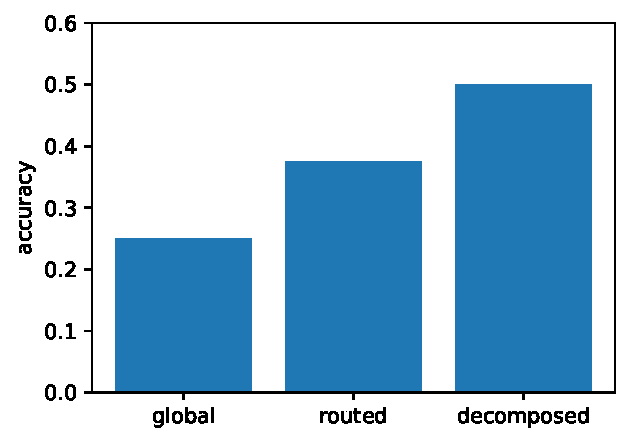
\includegraphics[width=0.65\linewidth]{figures/fig_router.pdf}
\caption{Router/decomposition accuracy on the disconnected additive set.}
\label{fig:router}
\end{figure}

\begin{table}[h]
\centering
\begin{tabular}{lr}
\toprule
mode & accuracy \\
\midrule
global & 25.0\% \\
routed & 37.5\% \\
decomposed & 50.0\% \\
\bottomrule
\end{tabular}

\caption{Router modes on the disconnected additive set.}
\label{tab:router}
\end{table}
% <<< AI-DRAFT

\end{document}
